% Permission is granted to copy, distribute and/or modify this document
% under the terms of the GNU Free Documentation License, Version 1.2
% or any later version published by the Free Software Foundation;
% with no Invariant Sections, no Front-Cover Texts, and no Back-Cover
% Texts.  A copy of the license is included in the section entitled "GNU
% Free Documentation License".
% Copyright 2016 EDF
%

%%%%%%%%%%%%%%%%%%%%%%%%%%%%%%%%%%%%%%%%%%%%%%%%%%%%%%%%%%%%%%%%%%%%%%%%%%%%%%%%%%%%%%%%%%
\section{Use cases}

\subsection{ANOVA table}

R listing
\begin{lstlisting}[style=RStyle]
# Output variables : weight of the plants
ctl <- c(4.17 ,5.58 ,5.18 ,6.11 ,4.50 ,4.61 ,5.17 ,4.53 , 5.33 ,5.14)
trt <- c(4.81 ,4.17 ,4.41 ,3.59 ,5.87 ,3.83 ,6.03 ,4.89 , 4.32 ,4.69)

# Input variables :
# - group " Ctl " : control group ( plant with standard conditions )
# - group " Trt " : Treatment group ( plant with nutritionally enriched environment )

group <- gl( 2, 10, 20, labels = c("Ctl","Trt"))
weight <- c(ctl,trt)

lm.D9 <- lm(weight ~ group)
summary(lm.D9)

### SAVE DATA
DATA = data.frame(cbind(ctl,trt))
names(DATA) = c("ctl","trt")
write.csv(DATA, file="DATA.csv",row.names=FALSE)
\end{lstlisting}

Output
\begin{lstlisting}[style=output]
Call:
lm(formula = weight ~ group)

Residuals:
    Min      1Q  Median      3Q     Max
-1.0710 -0.4938  0.0685  0.2462  1.3690

Coefficients:
            Estimate Std. Error t value Pr(>|t|)
(Intercept)   5.0320     0.2202  22.850 9.55e-15 ***
groupTrt     -0.3710     0.3114  -1.191    0.249
---
Signif. codes:  0 '***' 0.001 '**' 0.01 '*' 0.05 '.' 0.1 ' ' 1

Residual standard error: 0.6964 on 18 degrees of freedom
Multiple R-squared:  0.07308,   Adjusted R-squared:  0.02158
F-statistic: 1.419 on 1 and 18 DF,  p-value: 0.249
\end{lstlisting}

\newpage
Equivalent listing in python
\begin{lstlisting}[style=pythonStyle]
import openturns as ot

Sample = ot.NumericalSample.ImportFromTextFile("DATA.csv", ",")
ctl = Sample[:,0]
trt = Sample[:,1]

inputSample = ot.NumericalSample(ctl.getSize(), [0])
inputSample.add(ot.NumericalSample(trt.getSize(), [1]))
inputSample.setDescription(["Trt"])

outputSample = ctl
outputSample.add(trt)
outputSample.setDescription(["weight"])

algo = ot.LinearModelAlgorithm(inputSample, outputSample)
result = algo.getResult()
analysis = ot.LinearModelAnalysis(result)
print(analysis)
\end{lstlisting}

Output python
\begin{lstlisting}[style=output]
 Call:
Basis( [[Trt]->[1],[Trt]->[Trt]] )

 Coefficients:
             | Estimate    | Std Error   | t value     | Pr(>|t|)    | 
----------------------------------------------------------------------
[Trt]->[1]   | 5.032       | 0.220218    | 22.8501     | 9.54713e-15 | 
[Trt]->[Trt] | -0.371      | 0.311435    | -1.19126    | 0.249023    | 
----------------------------------------------------------------------

 Residual standard error: 0.69639 on 18 degrees of freedom 
 F-statistic: 1.4191 ,  p-value: 0.24822
----------------------------------
Multiple R-squared   | 0.0730776 | 
Adjusted R-squared   | 0.0215819 | 
----------------------------------

---------------------------------
Normality test       | p-value  | 
---------------------------------
Anderson-Darling     | 0.316615 | 
Chi-Squared          | 0.433749 | 
Kolmogorov-Smirnov   | 0.870208 | 
---------------------------------
\end{lstlisting}

\newpage
\subsection{Graphical diagnostics}

R listing
\begin{lstlisting}[style=RStyle]
require(stats)
require(graphics)
## Analysis of the life-cycle savings data
## given in Belsley, Kuh and Welsch.

LifeCycleSavings <- read.table('LifeCycleSavings.csv', header=TRUE, sep=",")

lm.model1 <- lm(sr ~ pop15 + pop75 + dpi + ddpi , data=LifeCycleSavings)
plot(lm.model1 , which =1:6)

lm.model2 <- lm(sr^4 ~ pop75 + dpi , data=LifeCycleSavings)
plot(lm.model2 , which =1:6)
\end{lstlisting}

Equivalent listing in python
\begin{lstlisting}[style=pythonStyle]
from openturns.viewer import View
import openturns as ot
import pandas as pd

# First column in this CSV file is country name, use
# pandas to easily filter it out.
data = pd.read_csv("LifeCycleSavings.csv", index_col=0)

Sample = ot.NumericalSample(data.values)
Sample.setName("LifeCycleSavings")
Sample.setDescription(["sr","pop15","pop75","dpi","ddpi"])

sr    = Sample[:,0]
pop15 = Sample[:,1]
pop75 = Sample[:,2]
dpi   = Sample[:,3]
ddpi  = Sample[:,4]

# model1
outputSample = Sample[:,0]
inputSample = Sample[:,1:5]

algo1 = ot.LinearModelAlgorithm(inputSample, outputSample)
result1 = algo1.getResult()
analysis1 = ot.LinearModelAnalysis(algo1.getResult())

for plot in ["drawResidualsVsFitted", "drawScaleLocation", "drawQQplot", "drawCookDistance", "drawResidualsVsLeverages", "drawCookVsLeverages"]:
    graph = getattr(analysis1, plot)()
    graph.draw("model1-"+plot, 640, 480)

# plot of residuals versus fitted values
graph = analysis1.drawResidualsVsFitted()
View(graph)

# scale-location plot of sqrt(|residuals|) versus fitted values
graph = analysis1.drawScaleLocation()
View(graph)

# Normal quantiles-quantiles plot of standardized residuals
graph = analysis1.drawQQplot()
View(graph)

# plot of Cook's distances versus row labels
graph = analysis1.drawCookDistance()
View(graph)

# plot of residuals versus leverages that adds bands corresponding to Cook's distances of 0.5 and 1
graph = analysis1.drawResidualsVsLeverages()
View(graph)

# plot of Cook's distances versus leverage/(1-leverage)
graph = analysis1.drawCookVsLeverages()
View(graph)

# model2
f = ot.NumericalMathFunction('x','x^4','y')
outputSample = f(sr)
inputSample = pop75
inputSample.stack(dpi)

algo2 = ot.LinearModelAlgorithm(inputSample, outputSample)
result2 = algo2.getResult()
analysis2 = ot.LinearModelAnalysis(algo2.getResult())

for plot in ["drawResidualsVsFitted", "drawScaleLocation", "drawQQplot", "drawCookDistance", "drawResidualsVsLeverages", "drawCookVsLeverages"]:
    graph = getattr(analysis2, plot)()
    graph.draw("model2-"+plot, 640, 480)

# plot of residuals versus fitted values
graph = analysis2.drawResidualsVsFitted()
View(graph)

# scale-location plot of sqrt(|residuals|) versus fitted values
graph = analysis2.drawScaleLocation()
View(graph)

# Normal quantiles-quantiles plot of standardized residuals
graph = analysis2.drawQQplot()
View(graph)

# plot of Cook's distances versus row labels
graph = analysis2.drawCookDistance()
View(graph)

# plot of residuals versus leverages that adds bands corresponding to Cook's distances of 0.5 and 1
graph = analysis2.drawResidualsVsLeverages()
View(graph)

# plot of Cook's distances versus leverage/(1-leverage)
graph = analysis2.drawCookVsLeverages()
View(graph)

\end{lstlisting}

\begin{figure}[p]
  \begin{center}
    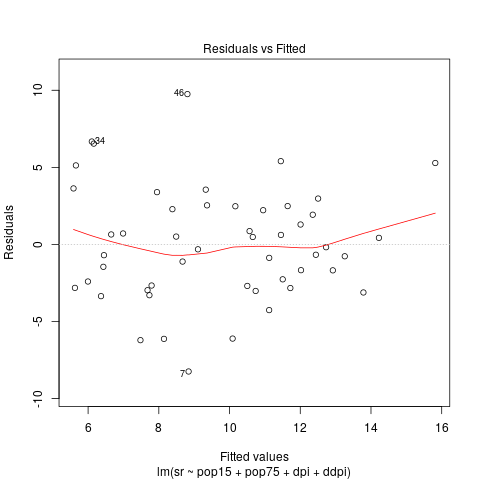
\includegraphics[scale=0.48]{imgR/plot11.png} \hspace*{2cm} 
	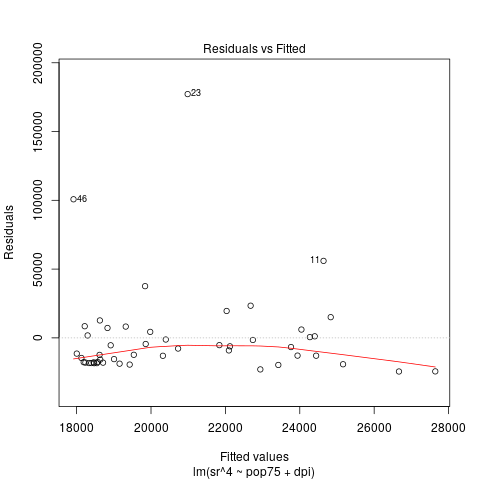
\includegraphics[scale=0.48]{imgR/plot21.png} \\
    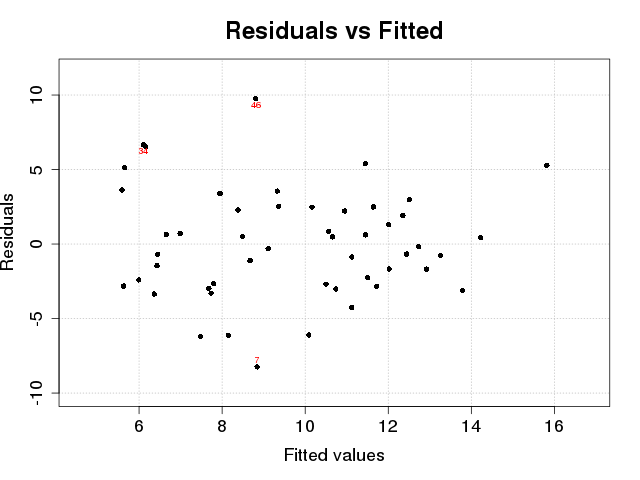
\includegraphics[scale=0.4]{imgOT/model1-drawResidualsVsFitted.png}\hspace*{1cm}
	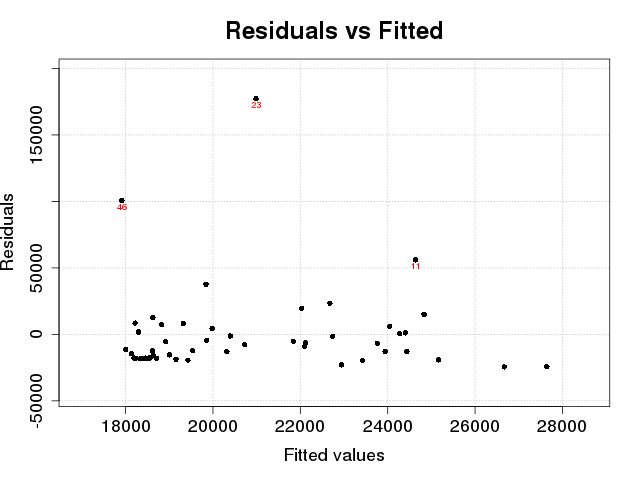
\includegraphics[scale=0.4]{imgOT/model2-drawResidualsVsFitted.png}\\
  \end{center}
  \caption{Residuals Vs Fitted}
\end{figure}

\begin{figure}[p]
  \begin{center}
    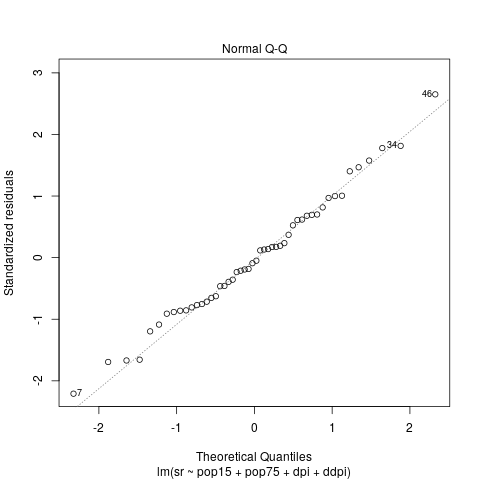
\includegraphics[scale=0.48]{imgR/plot12.png} \hspace*{2cm}
	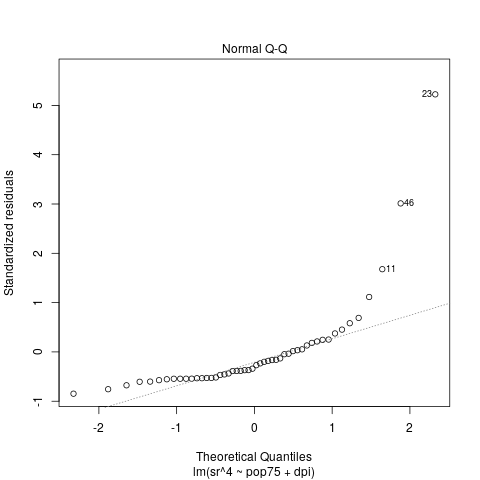
\includegraphics[scale=0.48]{imgR/plot22.png} \\
    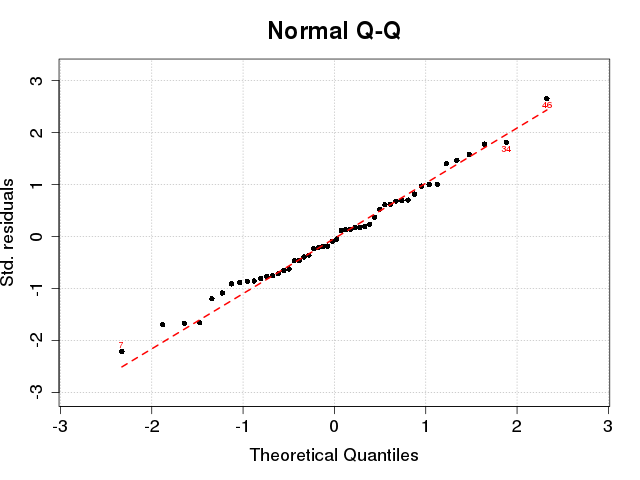
\includegraphics[scale=0.4]{imgOT/model1-drawQQplot.png}\hspace*{1cm}
	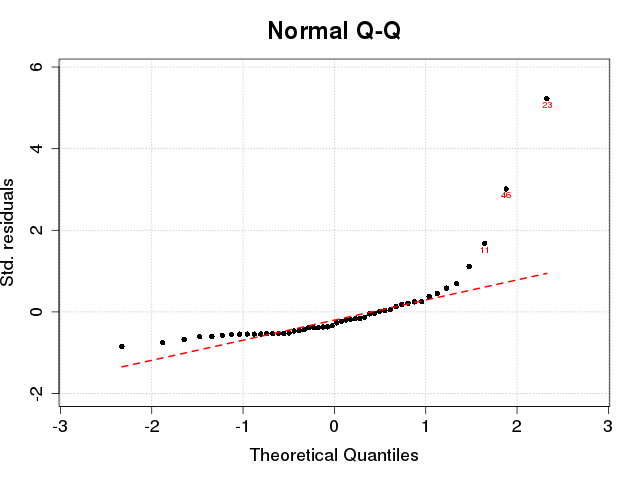
\includegraphics[scale=0.4]{imgOT/model2-drawQQplot.png}\\
  \end{center}
  \caption{Normal Q-Q}
\end{figure}

\begin{figure}[p]
  \begin{center}
    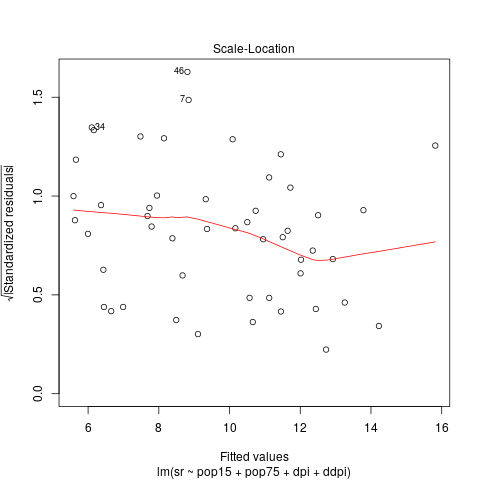
\includegraphics[scale=0.48]{imgR/plot13.png} \hspace*{2cm}
	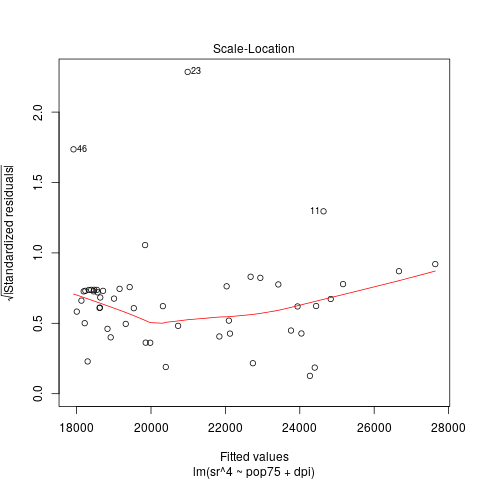
\includegraphics[scale=0.48]{imgR/plot23.png} \\
    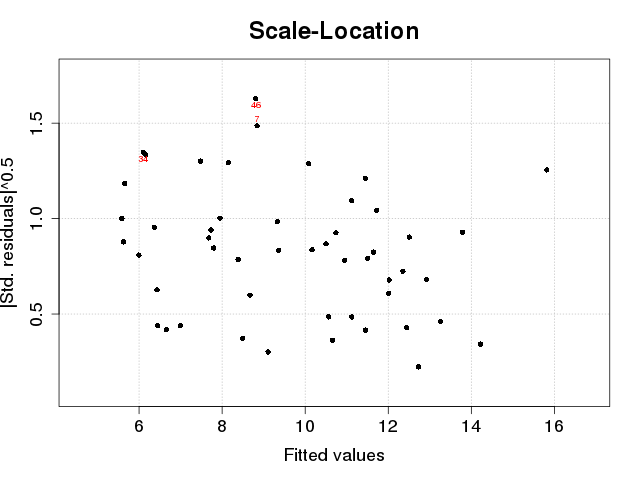
\includegraphics[scale=0.4]{imgOT/model1-drawScaleLocation.png}\hspace*{1cm}
	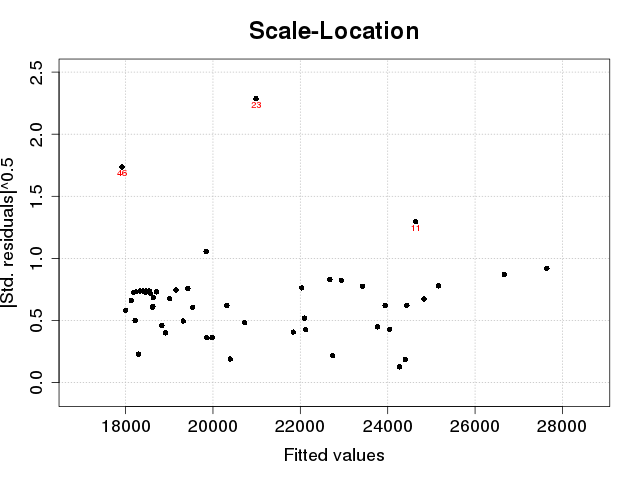
\includegraphics[scale=0.4]{imgOT/model2-drawScaleLocation.png}\\
  \end{center}
  \caption{Scale location}
\end{figure}

\begin{figure}[p]
  \begin{center}
    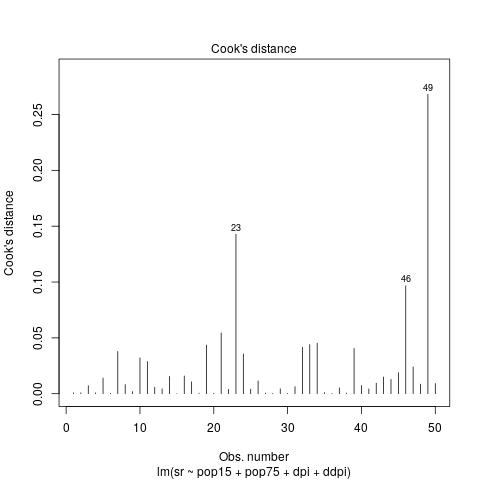
\includegraphics[scale=0.48]{imgR/plot14.png} \hspace*{2cm}
	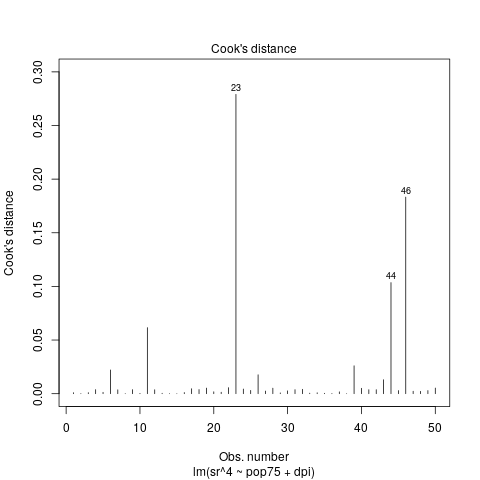
\includegraphics[scale=0.48]{imgR/plot24.png} \\
    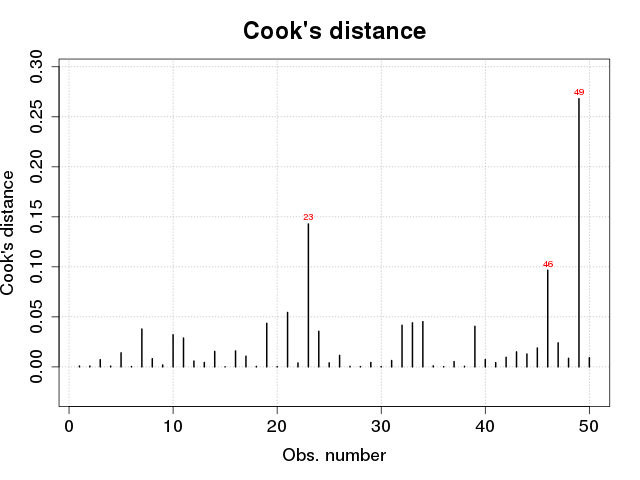
\includegraphics[scale=0.4]{imgOT/model1-drawCookDistance.png}\hspace*{1cm}
	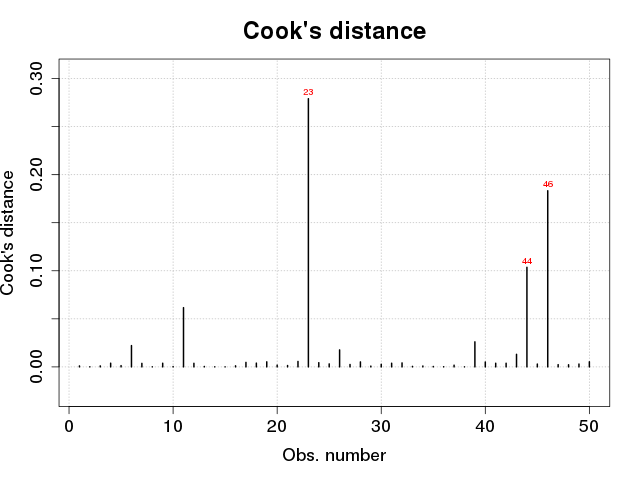
\includegraphics[scale=0.4]{imgOT/model2-drawCookDistance.png}\\
  \end{center}
  \caption{Cook's distance}
\end{figure}

\begin{figure}[p]
  \begin{center}
    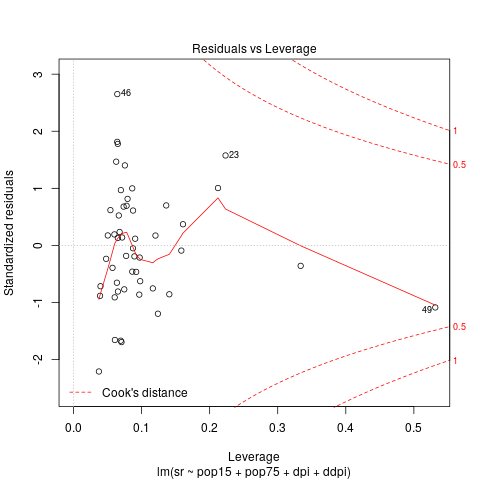
\includegraphics[scale=0.48]{imgR/plot15.png} \hspace*{2cm}
	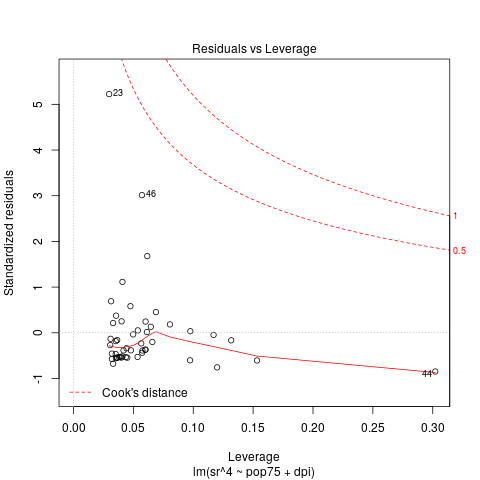
\includegraphics[scale=0.48]{imgR/plot25.png} \\
    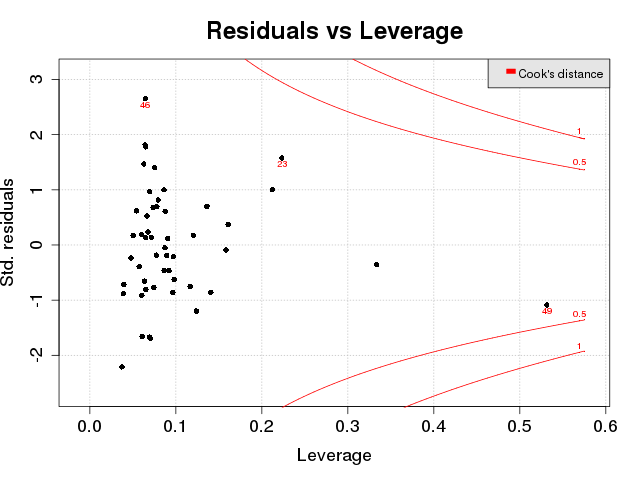
\includegraphics[scale=0.4]{imgOT/model1-drawResidualsVsLeverages.png}\hspace*{1cm}
	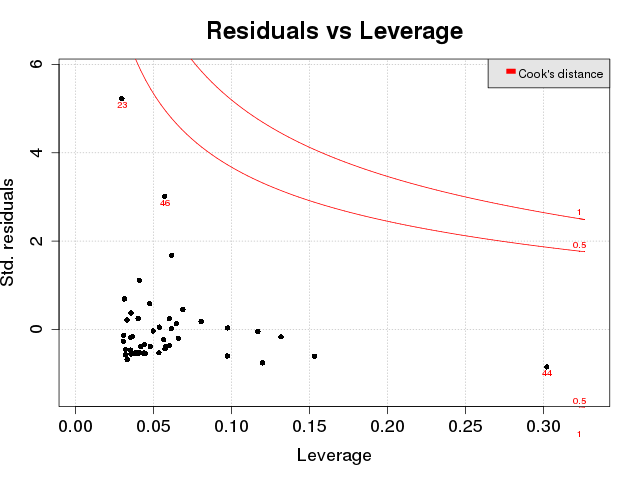
\includegraphics[scale=0.4]{imgOT/model2-drawResidualsVsLeverages.png}\\
  \end{center}
  \caption{Residuals Vs Leverages}
\end{figure}

\begin{figure}[p]
  \begin{center}
    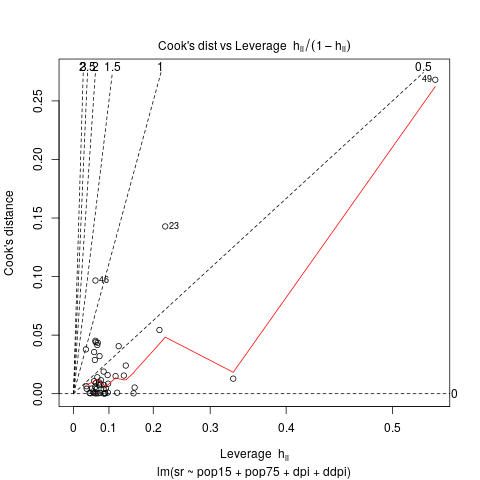
\includegraphics[scale=0.48]{imgR/plot16.png} \hspace*{2cm}
	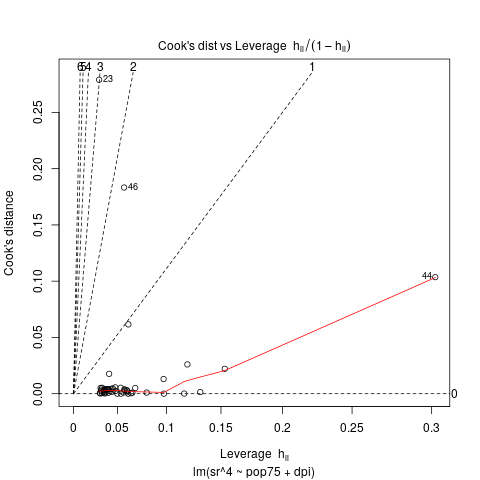
\includegraphics[scale=0.48]{imgR/plot26.png} \\
    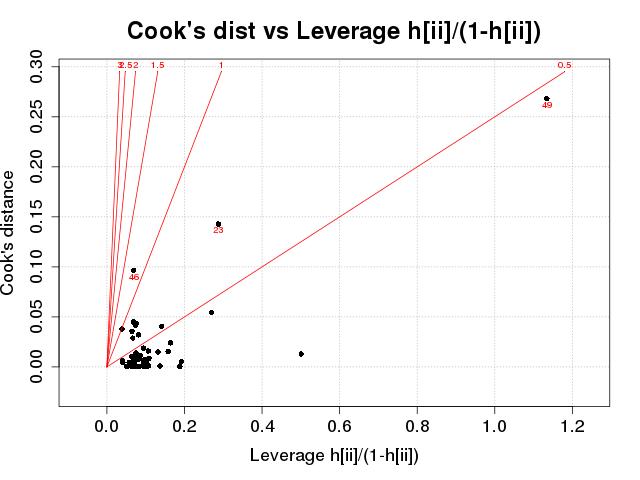
\includegraphics[scale=0.4]{imgOT/model1-drawCookVsLeverages.png}\hspace*{1cm}
	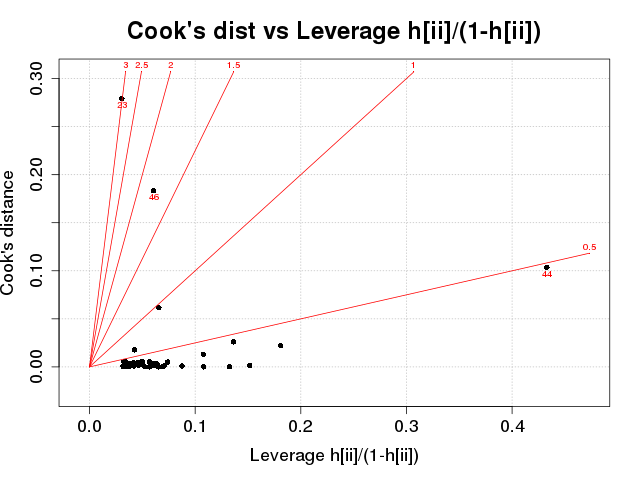
\includegraphics[scale=0.4]{imgOT/model2-drawCookVsLeverages.png}\\
  \end{center}
  \caption{Cook's distance Vs Leverages}
\end{figure}

\subsection{Step method}

R listing
\begin{lstlisting}[style=RStyle]
### DESIGN
X <- data.frame(cbind(X1,X2,X3,X4))
names(X) <- c("X1","X2","X3","X4")

### LINEAR MODEL
myLinearModel <- function(X) {
    beta <- c (14 , -7 , -17 , -7 , -3 ,13 , -16 , -4 ,12 ,3 ,13 ,20 ,17 , -10 ,7)
    Design <- cbind(rep(1,dim(X)[1]),X[,1],X[,2],X[,3],X[,4], X[,3]^2,X[,4]^2,X[,1]^2,X[,1]*X[,2],
                       X[,2]*X[,4] , X[,3]*X[,4] , X[,1]*X[,2]*X[,3] , X[,1]^3 ,X[,2]^3 ,X[,4]^3 )
    Y <- Design%*%as.matrix(beta)
    return(Y)
}

### OBSERVATIONS
Y <- myLinearModel(X) + residuals

### MIN/MAX/START MODELS
model_min <- lm(Y~1 , data=X)
model_max <- lm(Y~(X1+X2+X3+X4)^3+I(X1^2)+I(X1^3)+I(X2^2)+I(X2^3)
                                 +I(X3^2)+I(X3^3)+I(X4^2)+I(X4^3), data=X)
model_0 <- lm(Y~X1+X2+X3+X4 , data=X)


### STEPWISE PROCEDURE

## Forward
#AIC
lm_forward_AIC <- step( model_min , scope=list(lower=model_min , upper=model_max) , direction="forward" , k=2)
#BIC
lm_forward_BIC <- step( model_min , scope=list(lower=model_min , upper=model_max) , direction="forward" , k=log(100))


## Backward
#AIC
lm_backward_AIC <- step( model_max , scope=list(lower=model_min , upper=model_max) , direction="backward" , k=2)
#BIC
lm_backward_BIC <- step( model_max , scope=list(upper=model_max , lower=model_min) , direction="backward" , k=log(100))

## Both
#AIC
lm_both_AIC <- step( model_0 , scope=list(lower=model_min , upper=model_max) , direction="both" , k=2)
#BIC
lm_both_BIC <- step( model_0 , scope=list(upper=model_max , lower=model_min) , direction="both" , k=log(100))


### ANOVA
summary(lm_forward_AIC)
AIC(lm_forward_AIC)

summary(lm_forward_BIC)
BIC(lm_forward_BIC)

summary(lm_backward_AIC)
AIC(lm_backward_AIC)

summary(lm_backward_BIC)
BIC(lm_backward_BIC)

summary(lm_both_AIC)
AIC(lm_both_AIC)

summary(lm_both_BIC)
BIC(lm_both_BIC)
\end{lstlisting}

Output
\begin{lstlisting}[style=output]
> lm_forward_AIC <- step( model_min , scope=list(lower=model_min , upper=model_max) , direction="forward" , k=2)
Start:  AIC=435.91
Y ~ 1

          Df Sum of Sq    RSS    AIC
+ I(X1^3)  1   2449.82 5214.0 399.39
+ I(X1^2)  1   2449.50 5214.3 399.40
+ I(X3^3)  1   2368.07 5295.7 400.95
+ I(X3^2)  1   2196.96 5466.9 404.13
+ X1       1   2153.80 5510.0 404.92
+ X3       1   1758.18 5905.6 411.85
+ I(X2^3)  1   1647.84 6016.0 413.70
+ I(X2^2)  1   1529.15 6134.7 415.65
+ X2       1   1309.35 6354.5 419.17
<none>                 7663.8 435.91
+ X4       1     30.75 7633.1 437.51
+ I(X4^2)  1     19.71 7644.1 437.65
+ I(X4^3)  1      6.48 7657.3 437.82

Step:  AIC=399.39
Y ~ I(X1^3)

          Df Sum of Sq    RSS    AIC
+ I(X3^3)  1   1980.57 3233.4 353.61
+ I(X3^2)  1   1977.69 3236.3 353.70
+ X3       1   1755.95 3458.0 360.33
+ I(X2^3)  1   1490.22 3723.8 367.73
+ I(X2^2)  1   1456.80 3757.2 368.63
+ X2       1   1294.26 3919.7 372.86
+ X4       1    215.76 4998.2 397.17
+ I(X4^2)  1    185.36 5028.6 397.77
+ I(X4^3)  1    146.43 5067.6 398.54
<none>                 5214.0 399.39
+ I(X1^2)  1     16.24 5197.8 401.08
+ X1       1      4.00 5210.0 401.32

Step:  AIC=353.61
Y ~ I(X1^3) + I(X3^3)

          Df Sum of Sq    RSS    AIC
+ I(X2^3)  1   2314.62  918.8 229.79
+ I(X2^2)  1   2182.89 1050.5 243.19
+ X2       1   1837.77 1395.7 271.60
+ X4       1    413.32 2820.1 341.94
+ I(X4^2)  1    366.65 2866.8 343.58
+ I(X4^3)  1    313.41 2920.0 345.42
+ I(X1^2)  1    107.67 3125.8 352.23
<none>                 3233.4 353.61
+ X1       1     43.76 3189.7 354.25
+ I(X3^2)  1     12.71 3220.7 355.22
+ X3       1      7.47 3226.0 355.38

Step:  AIC=229.79
Y ~ I(X1^3) + I(X3^3) + I(X2^3)

          Df Sum of Sq    RSS    AIC
+ X4       1   250.068 668.74 200.02
+ I(X4^2)  1   248.890 669.92 200.20
+ I(X4^3)  1   230.851 687.96 202.86
+ X3       1    49.376 869.44 226.27
+ I(X3^2)  1    30.490 888.32 228.42
+ I(X1^2)  1    29.994 888.82 228.47
+ I(X2^2)  1    28.473 890.34 228.64
+ X2       1    24.443 894.37 229.09
<none>                 918.81 229.79
+ X1       1    17.215 901.60 229.90

Step:  AIC=200.02
Y ~ I(X1^3) + I(X3^3) + I(X2^3) + X4

          Df Sum of Sq    RSS    AIC
+ X3       1    68.112 600.63 191.28
+ I(X3^2)  1    54.472 614.27 193.53
+ I(X1^2)  1    18.731 650.01 199.18
<none>                 668.74 200.02
+ X1       1    10.555 658.19 200.43
+ I(X2^2)  1     5.174 663.57 201.25
+ X2       1     4.199 664.55 201.39
+ I(X4^2)  1     2.600 666.14 201.63
+ I(X4^3)  1     1.461 667.28 201.81

Step:  AIC=191.28
Y ~ I(X1^3) + I(X3^3) + I(X2^3) + X4 + X3

          Df Sum of Sq    RSS    AIC
+ X3:X4    1   132.222 468.41 168.42
+ I(X1^2)  1    13.201 587.43 191.06
<none>                 600.63 191.28
+ X1       1     8.781 591.85 191.81
+ I(X3^2)  1     7.303 593.33 192.06
+ I(X4^2)  1     5.537 595.10 192.35
+ I(X4^3)  1     4.005 596.63 192.61
+ X2       1     0.402 600.23 193.22
+ I(X2^2)  1     0.097 600.54 193.26

Step:  AIC=168.42
Y ~ I(X1^3) + I(X3^3) + I(X2^3) + X4 + X3 + X4:X3

          Df Sum of Sq    RSS    AIC
+ I(X4^2)  1   25.9297 442.48 164.72
+ I(X4^3)  1   25.5292 442.88 164.81
<none>                 468.41 168.42
+ I(X3^2)  1    4.6876 463.72 169.41
+ I(X1^2)  1    2.0693 466.34 169.97
+ X1       1    0.9149 467.50 170.22
+ I(X2^2)  1    0.7832 467.63 170.25
+ X2       1    0.3309 468.08 170.35

Step:  AIC=164.72
Y ~ I(X1^3) + I(X3^3) + I(X2^3) + X4 + X3 + I(X4^2) + X4:X3

          Df Sum of Sq    RSS    AIC
<none>                 442.48 164.72
+ I(X3^2)  1    4.0023 438.48 165.81
+ I(X1^2)  1    2.5372 439.94 166.15
+ X1       1    1.6099 440.87 166.36
+ I(X4^3)  1    0.0320 442.45 166.72
+ I(X2^2)  1    0.0249 442.46 166.72
+ X2       1    0.0014 442.48 166.72

...
\end{lstlisting}

Equivalent listing in python
\begin{lstlisting}[style=pythonStyle]
import openturns as ot
from math import log

Sample = ot.NumericalSample.ImportFromTextFile("DATA_test1.csv", ",")

X = Sample[:, 1:5]
R = Sample[:, 0]

myLinearModel = ot.NumericalMathFunction(['x1', 'x2', 'x3', 'x4'], ['y'],
    ['14 - 7*x1 - 17*x2 - 7 *x3 - 3*x4 + 13*x3^2 - 16*x4^2 ' +
       ' - 4*x1^2 + 12*x1*x2 + 3*x2*x4 + 13*x3*x4 + 20*x1*x2*x3 ' +
       ' + 17*x1^3 - 10*x2^3 + 7*x4^3'])

Y = myLinearModel(X) + R

penalty_BIC = log(X.getSize())
penalty_AIC = 2.
maxiteration = 1000

# Build a model Y~(X1+X2+X3+X4)^3+I(Xi)^2+I(Xi)^3
... Define basis, i_min and i_0

algo = ot.LinearModelStepwiseAlgorithm(X, basis, Y)
algo.setMinimalIndices(i_min)

## Forward
algo.setDirection(1)
algo.setPenalty(penalty_AIC)
lm_forward_AIC_result = algo.getResult()
algo.setPenalty(penalty_BIC)
lm_forward_BIC_result = algo.getResult()

## Backward
algo.setDirection(-1)
algo.setPenalty(penalty_AIC)
lm_backward_AIC_result = algo.getResult()
algo.setPenalty(penalty_BIC)
lm_backward_BIC_result = algo.getResult()

## Both
algo.setDirection(0)
algo.setPenalty(penalty_AIC)
algo.setStartIndices(i_0)
lm_both_AIC_result = algo.getResult()
algo.setPenalty(penalty_BIC)
lm_both_BIC_result = algo.getResult()

lm_forward_AIC_result.printANOVAtable()
lm_forward_BIC_result.printANOVAtable()

lm_backward_AIC_result.printANOVAtable()
lm_backward_BIC_result.printANOVAtable()

lm_both_AIC_result.printANOVAtable()
lm_both_BIC_result.printANOVAtable()
\end{lstlisting}

